\documentclass[a4paper]{article}
\usepackage[spanish]{babel}
\usepackage[utf8]{inputenc}
\usepackage{graphicx}
\usepackage{enumerate}
\usepackage{listings}
\usepackage{color}
\usepackage{indentfirst}
\usepackage{fancyhdr}
\usepackage{latexsym}
\usepackage[colorlinks=true, linkcolor=black]{hyperref}
%\usepackage{makeidx}
%\usepackage{float}
\usepackage{wrapfig}
\usepackage{calc}
\usepackage{amsmath, amsthm, amssymb}
\usepackage{amsfonts}
%\lstset{language=C}
\definecolor{gray}{gray}{0.5}
\definecolor{light-gray}{gray}{0.95}
\definecolor{orange}{rgb}{1,0.5,0}

\usepackage{fancyhdr}
\pagestyle{fancy}

%\renewcommand{\chaptermark}[1]{\markboth{#1}{}}
\renewcommand{\sectionmark}[1]{\markright{\thesection\ - #1}}

\fancyhf{}

\fancyhead[LO]{Sección \rightmark} % \thesection\ 
\fancyfoot[LO]{\small{Axel Straminsky, Jorge Quintana, Florencia Zanollo, Luis Toffoletti}}
\fancyfoot[RO]{\thepage}
\renewcommand{\headrulewidth}{0.5pt}
\renewcommand{\footrulewidth}{0.5pt}
\setlength{\hoffset}{-0.8in}
\setlength{\textwidth}{16cm}
%\setlength{\hoffset}{-1.1cm}
%\setlength{\textwidth}{16cm}
\setlength{\headsep}{0.5cm}
\setlength{\textheight}{25cm}
\setlength{\voffset}{-0.7in}
\setlength{\headwidth}{\textwidth}
\setlength{\headheight}{13.1pt}

\renewcommand{\baselinestretch}{1.1}  % line spacing


% \setcounter{secnumdepth}{2}
\usepackage{underscore}
\usepackage{caratula}
\usepackage{url}
\usepackage{float}
\usepackage{algorithm}
\usepackage[noend]{algpseudocode}





\newcommand{\cod}[1]{{\tt #1}}
\newcommand{\negro}[1]{{\bf #1}}
\newcommand{\ital}[1]{{\em #1}}
\newcommand{\may}[1]{{\sc #1}}
\newcommand{\tab}{\hspace*{2em}}

\hypersetup{
 pdfstartview= {FitH \hypercalcbp{\paperheight-\topmargin-1in-\headheight}},
 pdfauthor={Grupo},
 pdfsubject={Dise\~{n}o}
}

\lstdefinestyle{customc}{
  backgroundcolor=\color{light-gray},
  belowcaptionskip=1\baselineskip,
  breaklines=true,
  numbers=left,
  xleftmargin=\parindent,
  language=C,
  showstringspaces=false,
  basicstyle=\footnotesize\ttfamily,
  keywordstyle=\bfseries\color{blue},
  commentstyle=\itshape\color{gray},
  identifierstyle=\color{black},
  stringstyle=\color{orange},
}

\lstdefinestyle{customasm}{
  backgroundcolor=\color{light-gray},
  belowcaptionskip=1\baselineskip,
  numbers=left,
  xleftmargin=\parindent,
  language=[x86masm]Assembler,
  keywordstyle=\bfseries\color{blue},
  basicstyle=\footnotesize\ttfamily,
  commentstyle=\itshape\color{gray},
}

\lstset{escapechar=@}


\begin{document}

\thispagestyle{empty}
\materia{Teoría de las Comunicaciones}
\submateria{Segundo Cuatrimestre de 2016}
\titulo{TP 2: Rutas en Internet}
%\subtitulo{Scheduling}
\integrante{Axel Straminsky}{769/11}{axelstraminsky@gmail.com}
\integrante{Jorge Quintana}{}{}
\integrante{Florencia Zanollo}{934/11}{florenciazanollo@gmail.com}
\integrante{Luis Toffoletti}{827/11}{luis.toffoletti@gmail.com}

\makeatletter

\maketitle
\newpage

\thispagestyle{empty}
\vfill

\thispagestyle{empty}
\vspace{3cm}
\tableofcontents
\newpage

\newenvironment{myindentpar}[1]
{\begin{list}{1}
         {\setlength{\leftmargin}{#1}}
         \item[]
}
{\end{list} }

%\normalsize
\newpage

% -------------------------------------------------------
% Breve explicacion de la base teorica que fundamenta los metodos involucrados en el trabajo, junto con los metodos mismos.  
% -------------------------------------------------------

\section{Introducción}
El objetivo de este trabajo práctico es implementar nuestra propia versión de la herramienta \textit{traceroute}, y de esta manera estimar los enlaces tanto continentales como intercontinentales (submarinos) hacia distintas universidades del mundo. Además, analizamos posibles outliers[1] y anomalidades[2] en la ruta estimada.

\section{Desarrollo}

Para implementar la herramienta utilizamos la biblioteca Scapy. Utilizamos TTLs incrementales hasta un máximo de 30, y por cada valor de TTL enviamos un paquete ICMP hacia el host destino, y chequeamos si algún host nos envía una respuesta del tipo \textit{Time Exceeded}. Si este es el caso, quiere decir que se trata de un host intermedio (hop), y lo agregamos a la ruta estimada. Si el paquete respuesta es del tipo \textit{Echo Reply}, significa que llegamos al host destino. En ambos casos calculamos el RTT (Round Trip Time) del paquete enviado. Esto se realiza varias veces por cada TTL (en lo que llamamos \textit{ráfagas}), para de esta manera poder estimar un RRT promedio para cada hop.

Si obtuvimos una respuesta en una o más ráfagas, calculamos el $\Delta RTT$, que se define como

$\Delta RTT_{i} = RTT_{i} - RTT_{i-1}$ donde $RTT_{i}$ es el $RTT$ promediado de todas las ráfagas enviadas hacia un hop.

Adicionalmente, utilizamos un web service de geolocalización [3] para estimar el país, ciudad, latitud y longitud del hop, y de esta manera ser capaces de ubicarlos en un mapa.
\newpage

\section{Resultados}
A continuación se detalla la información obtenida de las mediciones con cada universidad elegida.

\subsection{Universidad de San Petersburgo}

Resultados obtenidos en el monitoreo:\\

\smallskip
\begin{tabular}{| l | c | c | c | c |}
\hline
Hop & IP &  RTT promedio (s)  & deltaRTT promedio & Ubicacion\\ 
\hline
1 & 192.168.11.1 & 0.01142361429 & 0.01142361429 & Argentina, Buenos Aires\\
\hline
2 & 10.21.128.1 & 0.0283621417152 & 0.0169385274251 & Argentina, Buenos Aires\\
\hline
3 & 10.242.0.201 & 0.0378749105665 & 0.00951276885139 & Argentina, Buenos Aires\\
\hline
4 & 195.22.220.33 & 0.0143795543247 & 0 & Italy\\
\hline
5 & 195.22.220.32 & 0.292960882187 & 0.278581327862 & Italy\\
\hline
6 & 89.221.41.171 & 0.152727180057 & 0 & Italy\\
\hline
7 & 89.221.41.171 & 0.156960460875 & 0.00423328081767 & Italy\\
\hline
8 & 154.54.9.17 & 0.202791770299 & 0.0458313094245 & United States\\
\hline
9 & 154.54.80.41 & 0.21254154614 & 0.00974977584112 & United States\\
\hline
10 & 66.28.4.237 & 0.168935351902 & 0 & United States, Pasadena\\
\hline
11 & 154.54.29.222 & 0.251122385263 & 0.0821870333619 & United States\\
\hline
12 & 154.54.42.77 & 0.316137870153 & 0.0650154848893 & United States\\
\hline
13 & 154.54.45.162 & 0.327892038557 & 0.0117541684045 & United States\\
\hline
14 & 154.54.45.2 & 0.255609459347 & 0 & United States\\
\hline
15 & 38.88.196.186 & 0.270633061727 & 0.0150236023797 & United States, Los Angeles\\
\hline
16 & 101.4.117.169 & 0.435372935401 & 0.164739873674 & China, Beijing\\
\hline
17 & 101.4.117.97 & 0.467933893204 & 0.0325609578027 & China, Beijing\\
\hline
18 & 101.4.112.105 & 0.437322590086 & 0 & China, Beijing\\
\hline
19 & 101.4.118.94 & 0.43985332383 & 0.0025307337443 & China, Beijing\\
\hline
20 & 101.4.112.90 & 0.435603486167 & 0 & China, Beijing\\
\hline
21 & 101.4.117.81 & 0.413042836719 & 0 & China, Beijing\\
\hline
22 & 202.112.41.178 & 0.405184189479 & 0 & China, Shanghai\\
\hline
23 & 202.112.41.182 & 0.394645796882 & 0 & China, Shanghai\\
\hline
24 & 162.105.252.133 & 0.488684309853 & 0.0940385129717 & China, Beijing\\
\hline
\end{tabular}
\bigskip

\textbf{Paquetes enviados: 145 / Paquetes no respondidos: 14}\\

\textbf{Dos outliers, hops: 10 y 11}\\

Algo extraño es que según la herramienta de geolocalización los saltos 7 a 9 están ubicados en España, no creemos que esto sea así ya que sus RTT promedio son muy parecidos a los de Argentina. Esto lo reflejamos en el gráfico del planisferio.\\

En el hop 10 aumenta el RTT promedio (y es un outlier) ya que es entonces en donde suponemos viaja hasta Estados Unidos. El hop 11 no varía demasiado respecto al 10 y a pesar de ser un outlier no es un salto importante, no se viaja intercontinentalmente, como en el próximo (el hop 12) en el cual se llega hasta Irlanda.\\

Después de ese salto los RTT se mantienen entre si, ninguno se destaca, hasta llegar a destino. Con esto vemos que el método Cimbala en este caso falla al detectar el salto intercontinental.\\

A continuación mostramos un gráfico con los RTT entre saltos y otro con los ZRTT\footnote{ZRTT = $(X_i - \bar{X}) / S$}  entre saltos. También así el planisferio con los saltos graficados.

\begin{center}
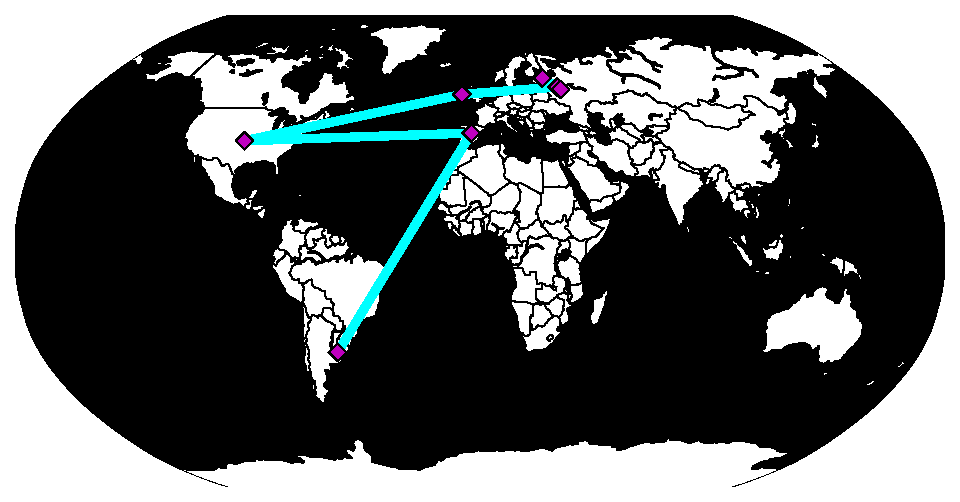
\includegraphics[scale=0.8]{imagenes/rusia/rusia.pdf} 
\end{center}


\subsection{Universidad de Pekín}

Resultados obtenidos en el monitoreo:\\

\smallskip
\begin{tabular}{| l | c | c | c | c |}
\hline
Hop & IP &  RTT promedio (s)  & deltaRTT promedio & Ubicacion\\ 
\hline
1 & 192.168.11.1 & 0.01142361429 & 0.01142361429 & Argentina, Buenos Aires\\
\hline
2 & 10.21.128.1 & 0.0283621417152 & 0.0169385274251 & Argentina, Buenos Aires\\
\hline
3 & 10.242.0.201 & 0.0378749105665 & 0.00951276885139 & Argentina, Buenos Aires\\
\hline
4 & 195.22.220.33 & 0.0143795543247 & 0 & Italy\\
\hline
5 & 195.22.220.32 & 0.292960882187 & 0.278581327862 & Italy\\
\hline
6 & 89.221.41.171 & 0.152727180057 & 0 & Italy\\
\hline
7 & 89.221.41.171 & 0.156960460875 & 0.00423328081767 & Italy\\
\hline
8 & 154.54.9.17 & 0.202791770299 & 0.0458313094245 & United States\\
\hline
9 & 154.54.80.41 & 0.21254154614 & 0.00974977584112 & United States\\
\hline
10 & 66.28.4.237 & 0.168935351902 & 0 & United States, Pasadena\\
\hline
11 & 154.54.29.222 & 0.251122385263 & 0.0821870333619 & United States\\
\hline
12 & 154.54.42.77 & 0.316137870153 & 0.0650154848893 & United States\\
\hline
13 & 154.54.45.162 & 0.327892038557 & 0.0117541684045 & United States\\
\hline
14 & 154.54.45.2 & 0.255609459347 & 0 & United States\\
\hline
15 & 38.88.196.186 & 0.270633061727 & 0.0150236023797 & United States, Los Angeles\\
\hline
16 & 101.4.117.169 & 0.435372935401 & 0.164739873674 & China, Beijing\\
\hline
17 & 101.4.117.97 & 0.467933893204 & 0.0325609578027 & China, Beijing\\
\hline
18 & 101.4.112.105 & 0.437322590086 & 0 & China, Beijing\\
\hline
19 & 101.4.118.94 & 0.43985332383 & 0.0025307337443 & China, Beijing\\
\hline
20 & 101.4.112.90 & 0.435603486167 & 0 & China, Beijing\\
\hline
21 & 101.4.117.81 & 0.413042836719 & 0 & China, Beijing\\
\hline
22 & 202.112.41.178 & 0.405184189479 & 0 & China, Shanghai\\
\hline
23 & 202.112.41.182 & 0.394645796882 & 0 & China, Shanghai\\
\hline
24 & 162.105.252.133 & 0.488684309853 & 0.0940385129717 & China, Beijing\\
\hline
\end{tabular}
\bigskip

\textbf{Paquetes enviados: 261 / Paquetes no respondidos: 48}\\

\textbf{Ocho outliers, hops: 5, 8, 11, 12, 15, 16, 17 y 24}\\

[INSERTE ANÁLISIS AQUÍ]

A continuación mostramos un gráfico con los RTT entre saltos y otro con los ZRTT\footnote{ZRTT = $(X_i - \bar{X}) / S$}  entre saltos. También así el planisferio con los saltos graficados.

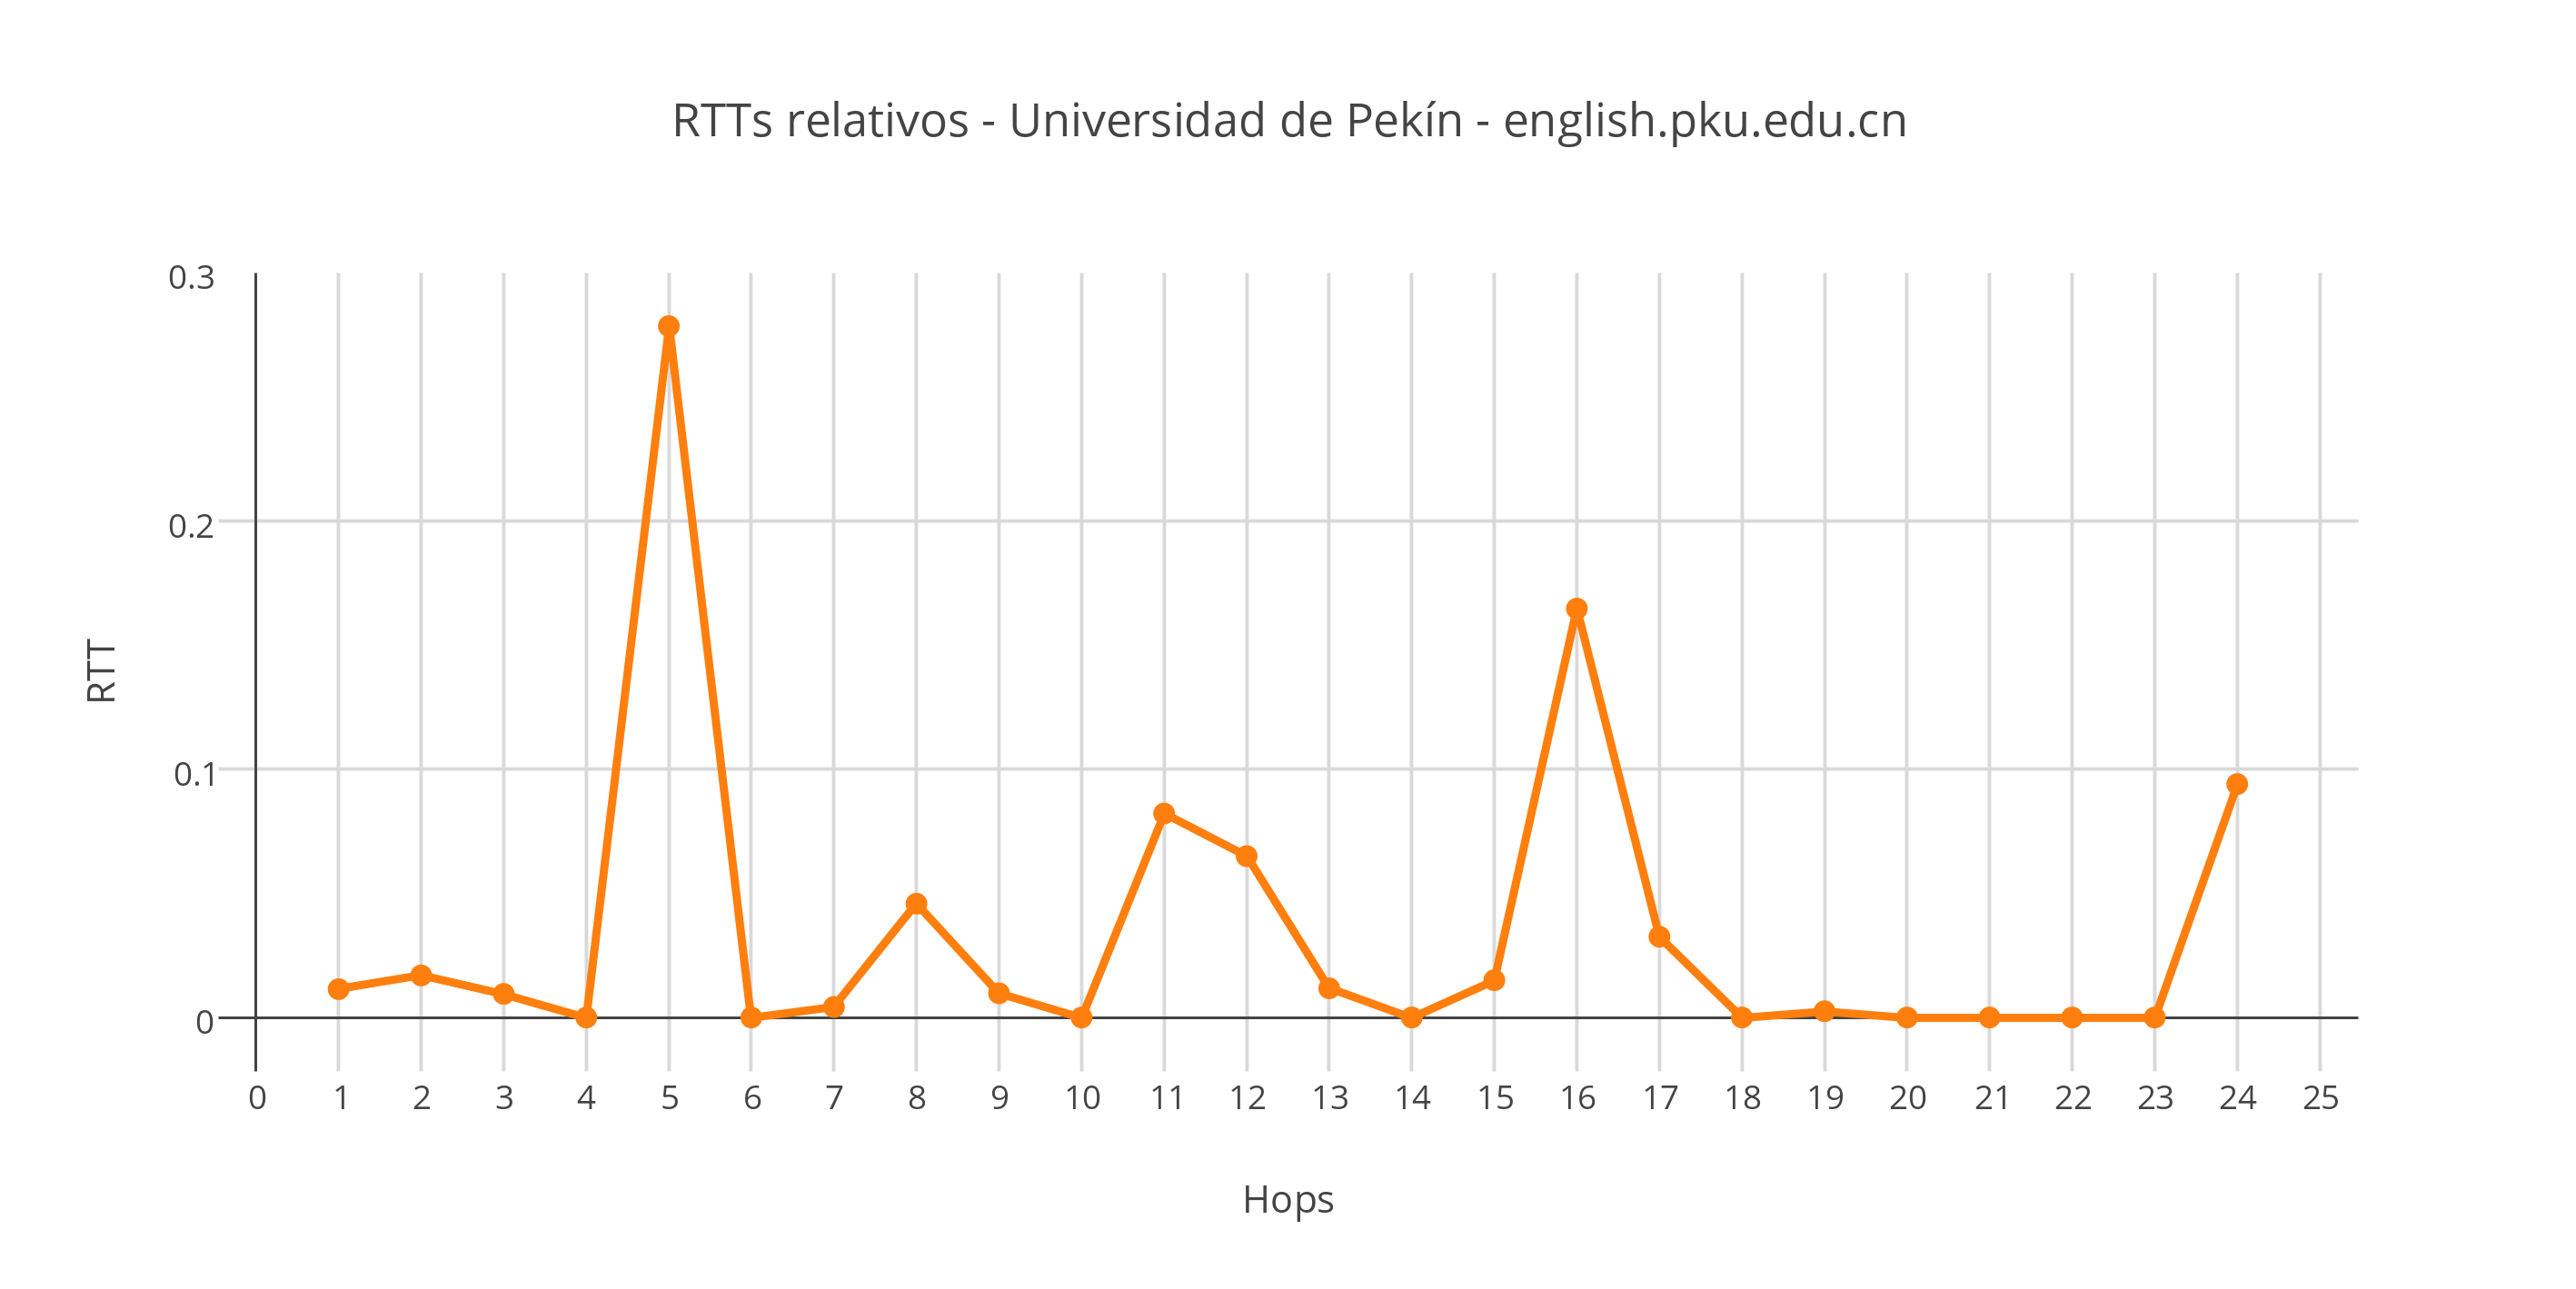
\includegraphics[scale=0.65]{imagenes/pekin/RTTs.png} 

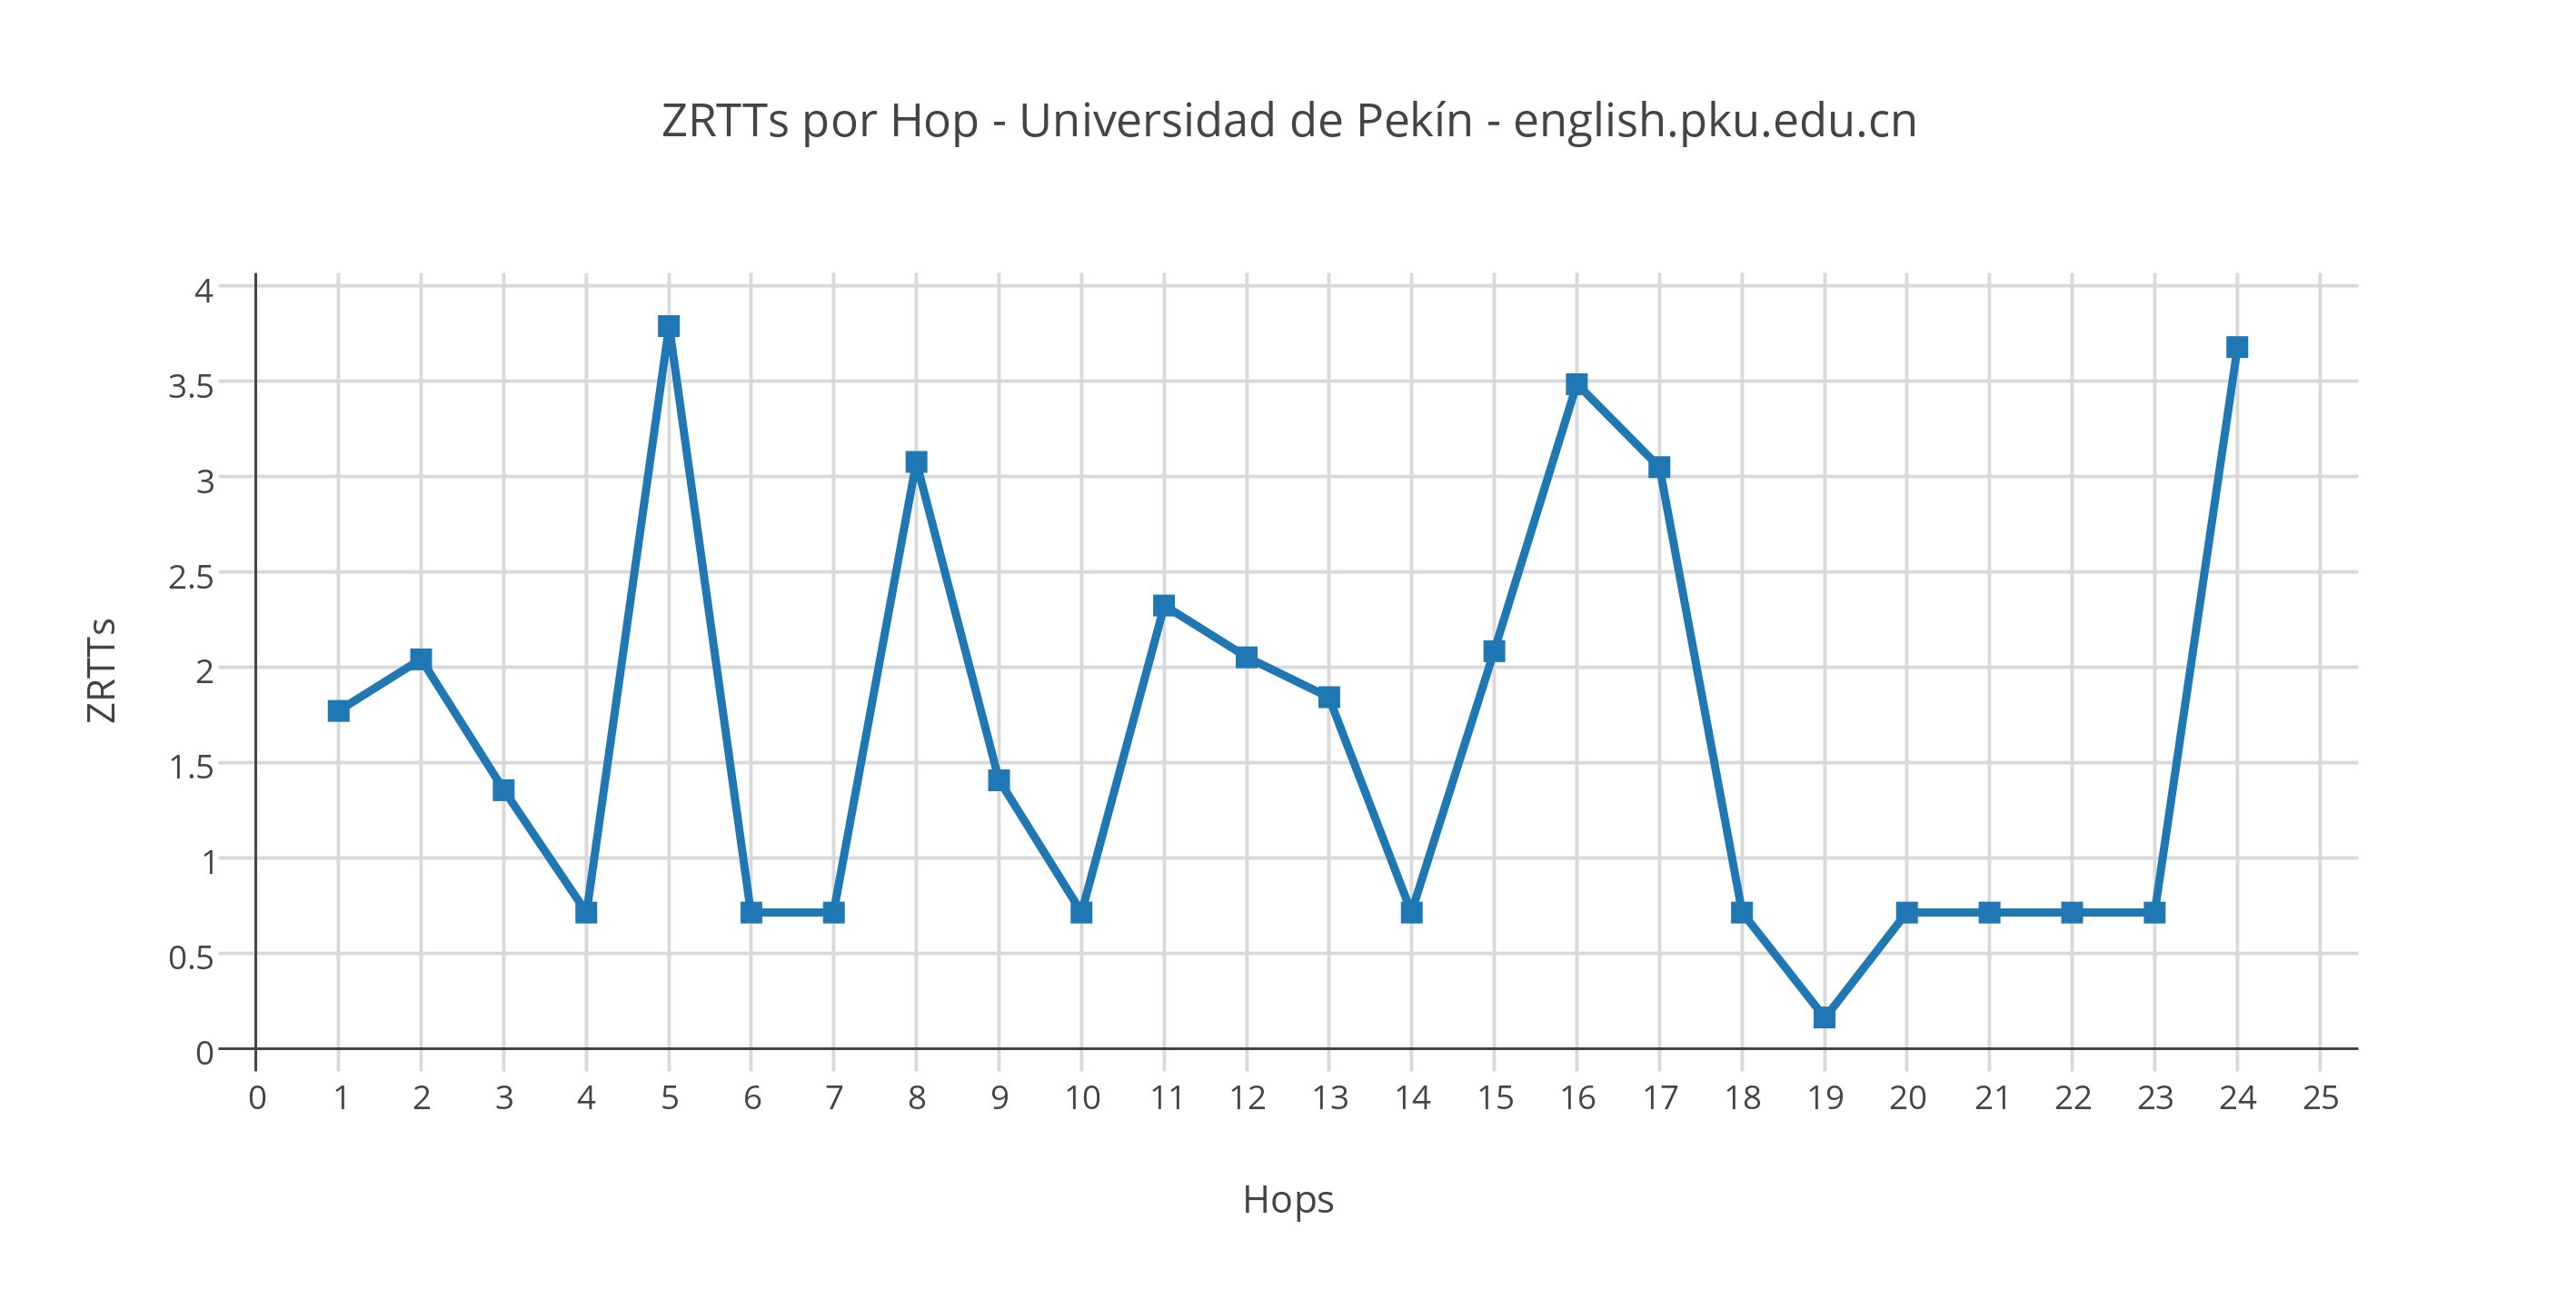
\includegraphics[scale=0.65]{imagenes/pekin/ZRTTs.png} 

\begin{center}
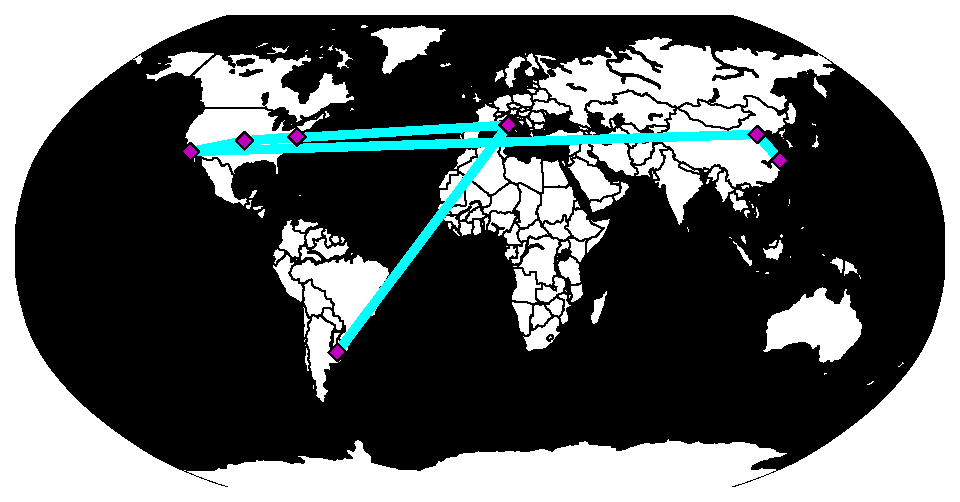
\includegraphics[scale=0.8]{imagenes/pekin/pekin.pdf} 
\end{center}


\subsection{Universidad de Helsinki}

Resultados obtenidos en el monitoreo:\\

\smallskip
\begin{tabular}{| l | c | c | c | c |}
\hline
Hop & IP &  RTT promedio (s)  & deltaRTT promedio & Ubicacion\\ 
\hline
1 & 192.168.11.1 & 0.01142361429 & 0.01142361429 & Argentina, Buenos Aires\\
\hline
2 & 10.21.128.1 & 0.0283621417152 & 0.0169385274251 & Argentina, Buenos Aires\\
\hline
3 & 10.242.0.201 & 0.0378749105665 & 0.00951276885139 & Argentina, Buenos Aires\\
\hline
4 & 195.22.220.33 & 0.0143795543247 & 0 & Italy\\
\hline
5 & 195.22.220.32 & 0.292960882187 & 0.278581327862 & Italy\\
\hline
6 & 89.221.41.171 & 0.152727180057 & 0 & Italy\\
\hline
7 & 89.221.41.171 & 0.156960460875 & 0.00423328081767 & Italy\\
\hline
8 & 154.54.9.17 & 0.202791770299 & 0.0458313094245 & United States\\
\hline
9 & 154.54.80.41 & 0.21254154614 & 0.00974977584112 & United States\\
\hline
10 & 66.28.4.237 & 0.168935351902 & 0 & United States, Pasadena\\
\hline
11 & 154.54.29.222 & 0.251122385263 & 0.0821870333619 & United States\\
\hline
12 & 154.54.42.77 & 0.316137870153 & 0.0650154848893 & United States\\
\hline
13 & 154.54.45.162 & 0.327892038557 & 0.0117541684045 & United States\\
\hline
14 & 154.54.45.2 & 0.255609459347 & 0 & United States\\
\hline
15 & 38.88.196.186 & 0.270633061727 & 0.0150236023797 & United States, Los Angeles\\
\hline
16 & 101.4.117.169 & 0.435372935401 & 0.164739873674 & China, Beijing\\
\hline
17 & 101.4.117.97 & 0.467933893204 & 0.0325609578027 & China, Beijing\\
\hline
18 & 101.4.112.105 & 0.437322590086 & 0 & China, Beijing\\
\hline
19 & 101.4.118.94 & 0.43985332383 & 0.0025307337443 & China, Beijing\\
\hline
20 & 101.4.112.90 & 0.435603486167 & 0 & China, Beijing\\
\hline
21 & 101.4.117.81 & 0.413042836719 & 0 & China, Beijing\\
\hline
22 & 202.112.41.178 & 0.405184189479 & 0 & China, Shanghai\\
\hline
23 & 202.112.41.182 & 0.394645796882 & 0 & China, Shanghai\\
\hline
24 & 162.105.252.133 & 0.488684309853 & 0.0940385129717 & China, Beijing\\
\hline
\end{tabular}
\bigskip

\textbf{Paquetes enviados: 407 / Paquetes no respondidos: 37}\\

\textbf{Tres outliers, hops: 4, 6 y 8}\\

[INSERTE ANÁLISIS AQUÍ]

A continuación mostramos un gráfico con los RTT entre saltos y otro con los ZRTT\footnote{ZRTT = $(X_i - \bar{X}) / S$}  entre saltos. También así el planisferio con los saltos graficados.

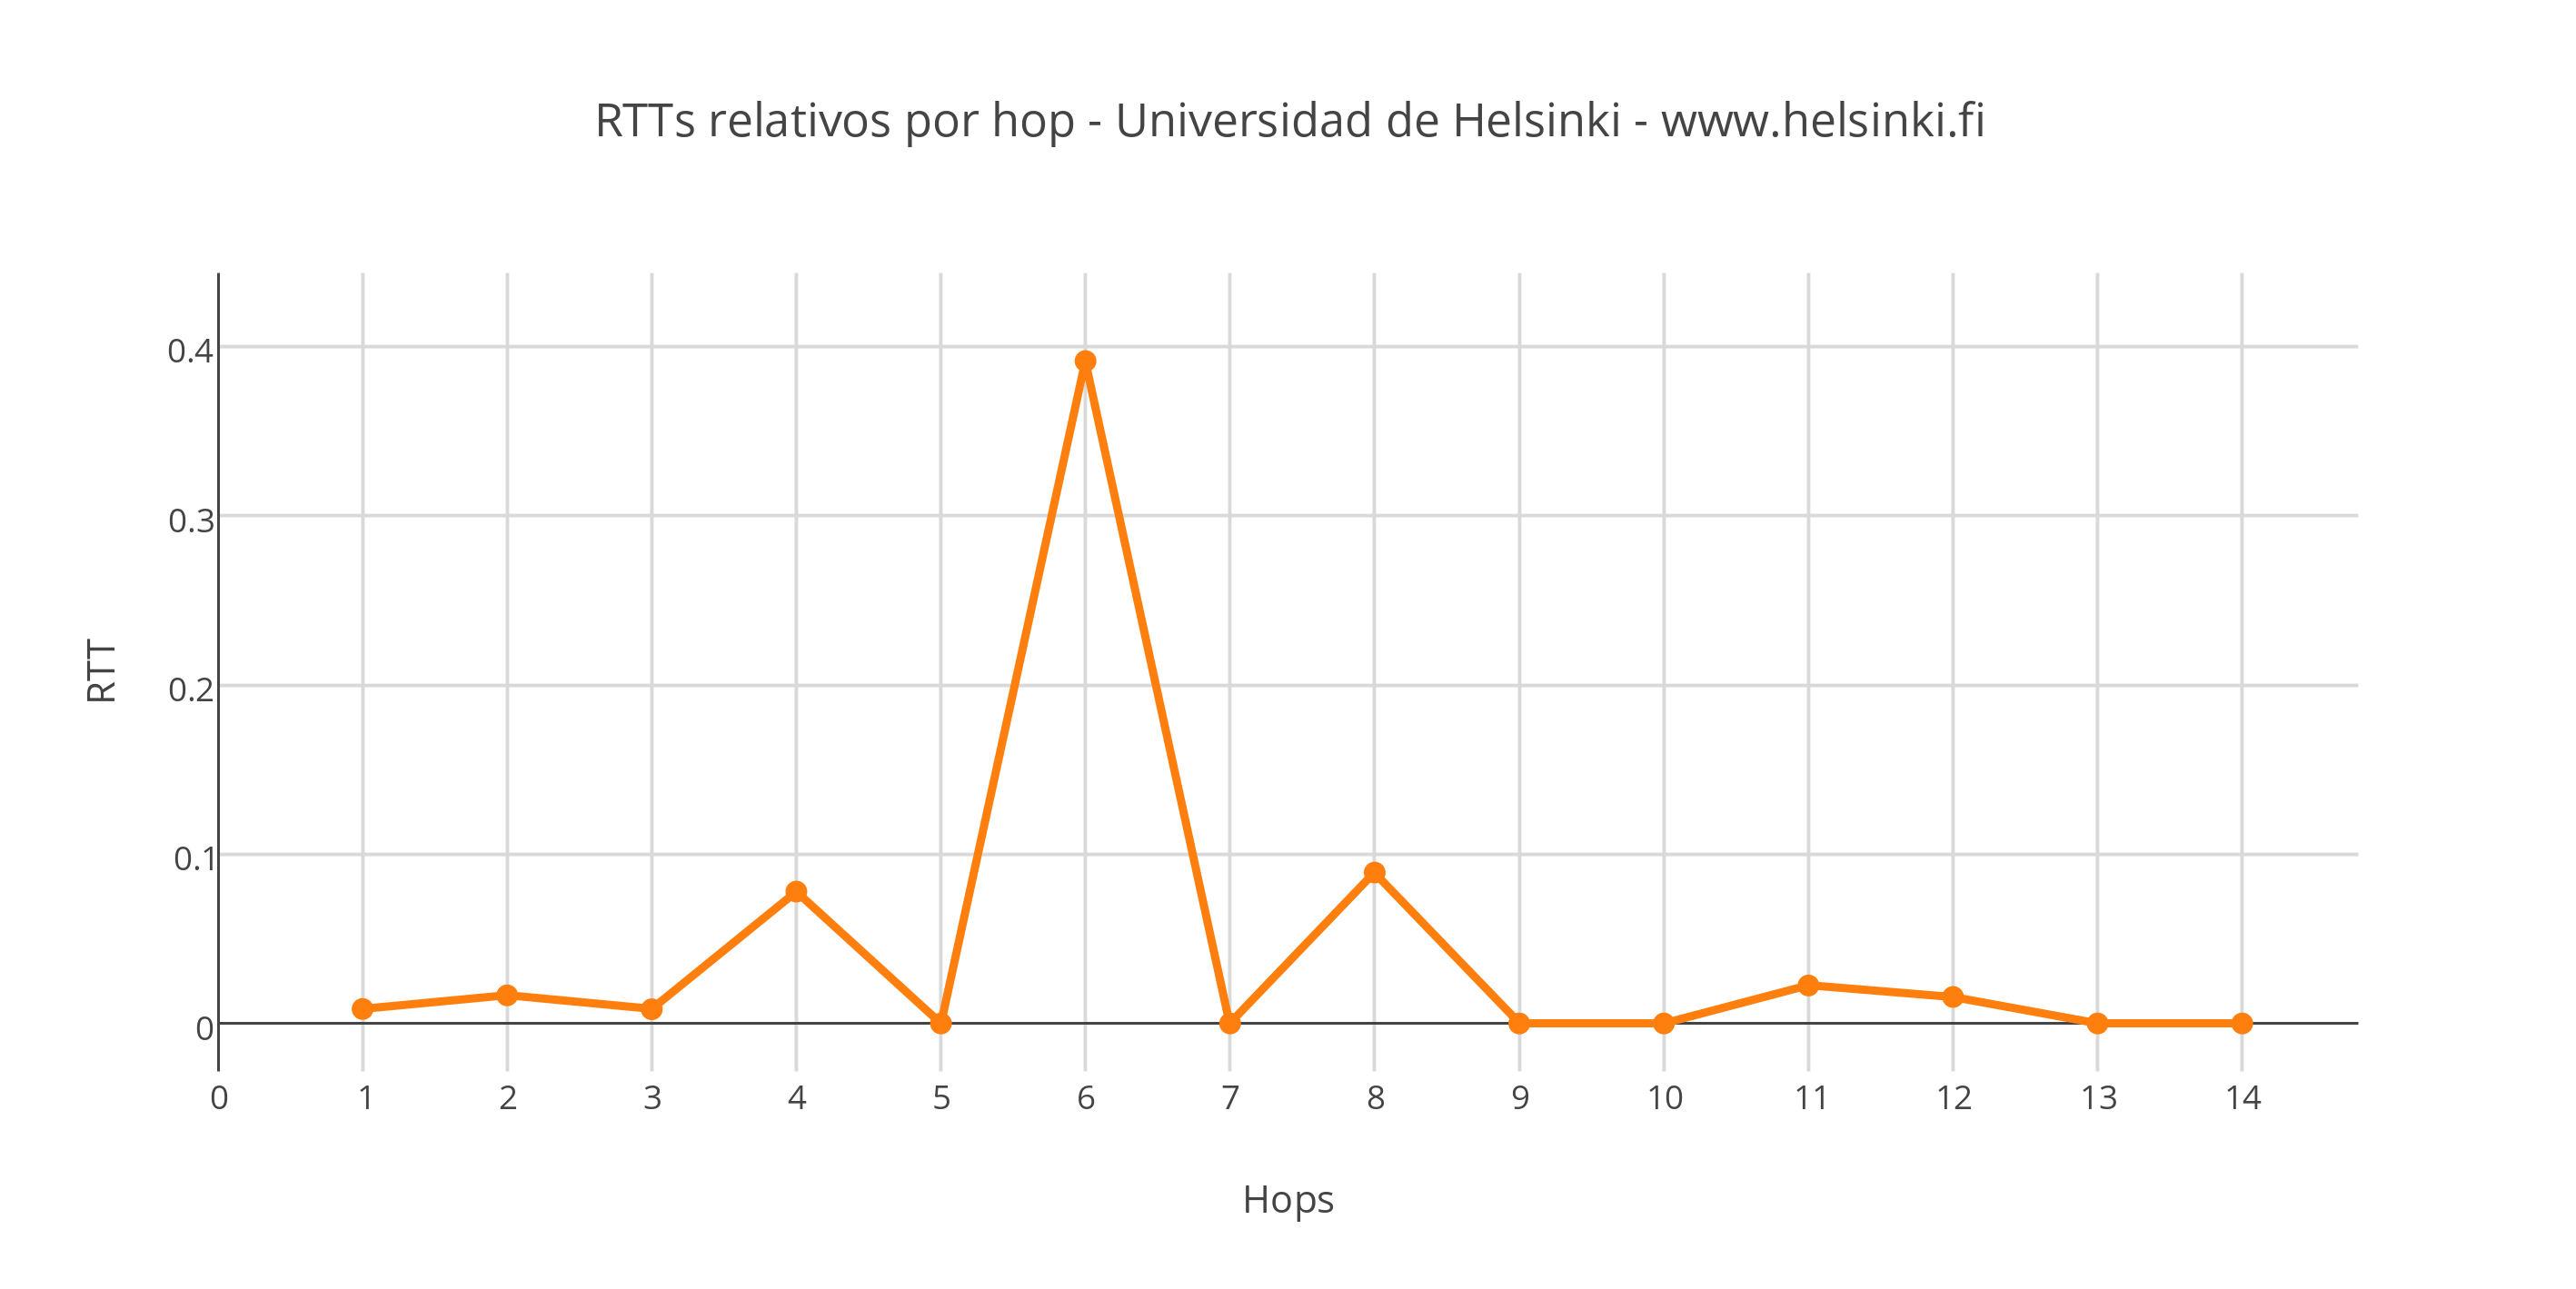
\includegraphics[scale=0.65]{imagenes/helsinki/RTTs.png} 

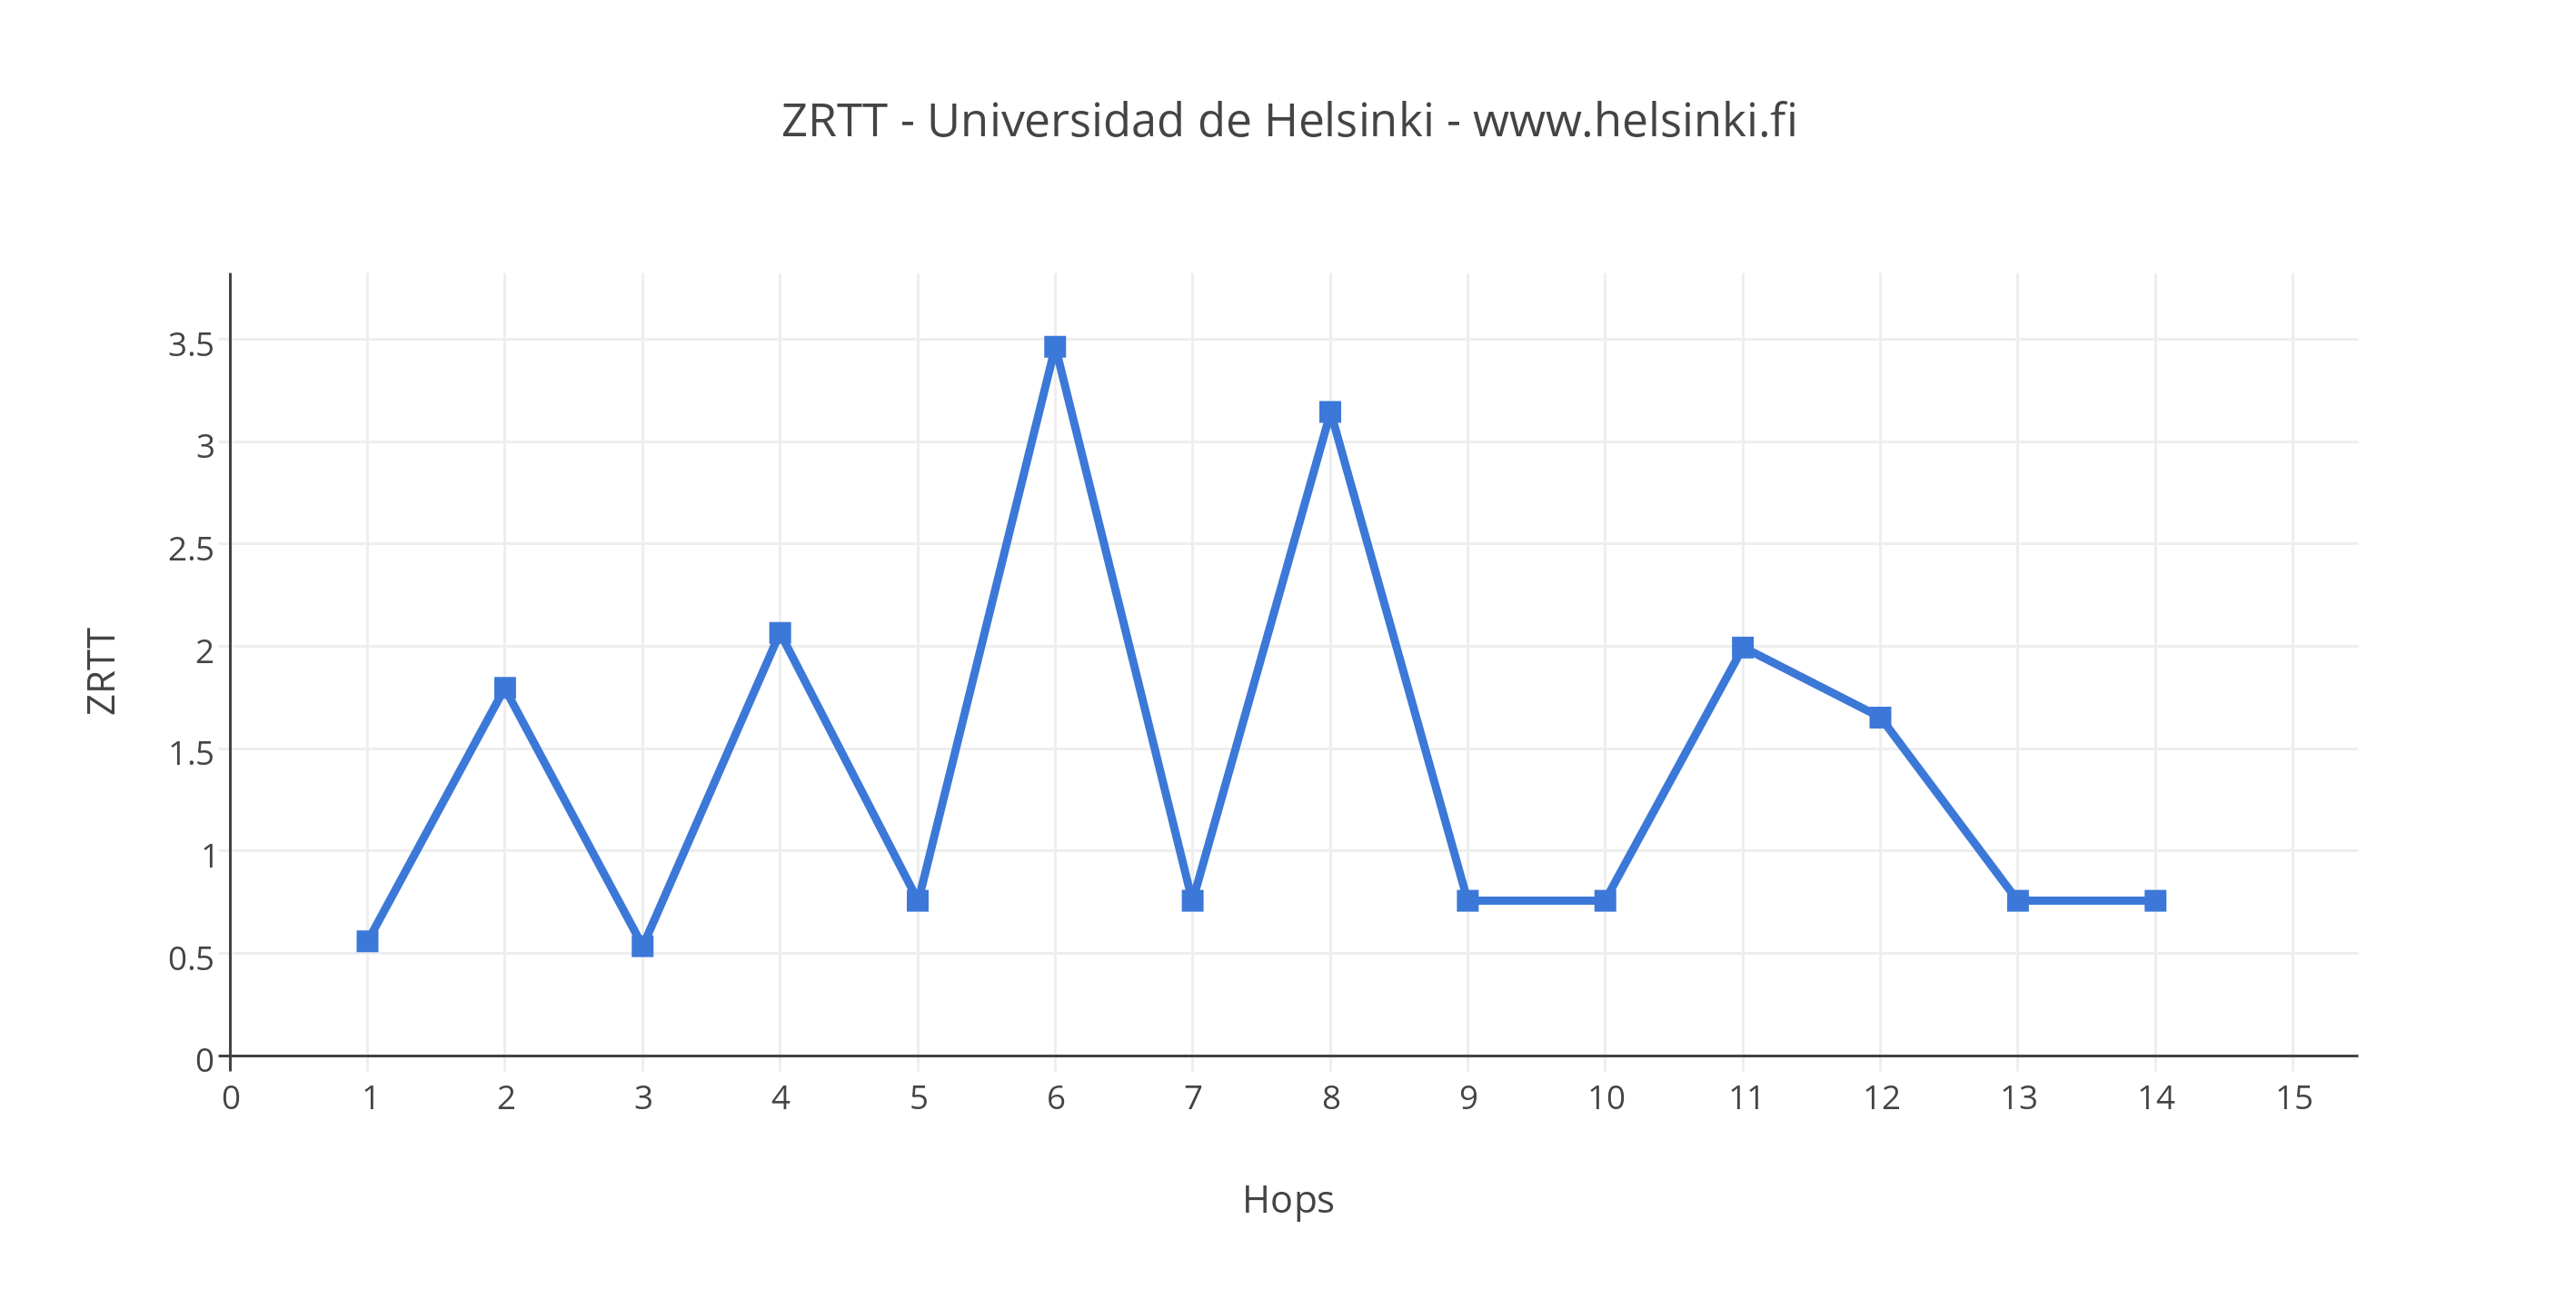
\includegraphics[scale=0.65]{imagenes/helsinki/ZRTTs.png} 

\begin{center}
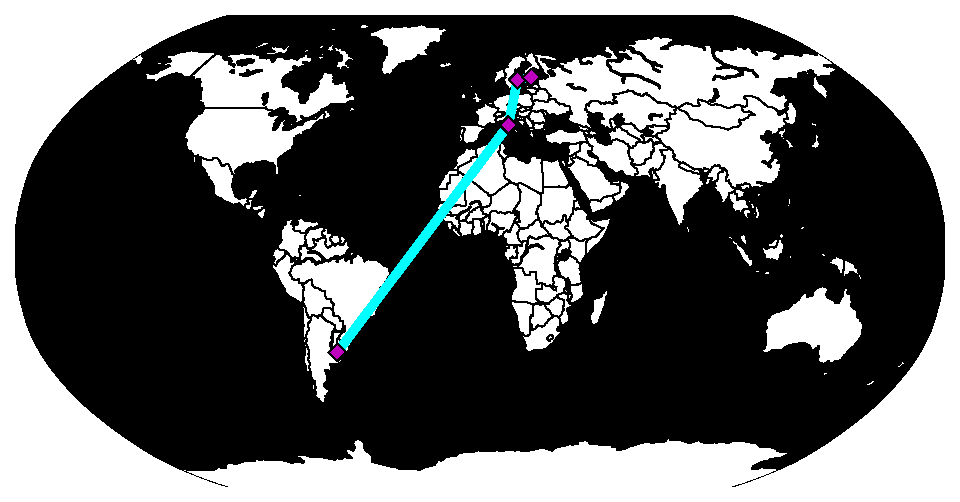
\includegraphics[scale=0.8]{imagenes/helsinki/helsinki.pdf} 
\end{center}

\subsection{Universidad de Sudáfrica}

Resultados obtenidos en el monitoreo:\\

\smallskip
\begin{tabular}{| l | c | c | c | c |}
\hline
Hop & IP &  RTT promedio (s)  & deltaRTT promedio & Ubicacion\\ 
\hline
1 & 192.168.11.1 & 0.01142361429 & 0.01142361429 & Argentina, Buenos Aires\\
\hline
2 & 10.21.128.1 & 0.0283621417152 & 0.0169385274251 & Argentina, Buenos Aires\\
\hline
3 & 10.242.0.201 & 0.0378749105665 & 0.00951276885139 & Argentina, Buenos Aires\\
\hline
4 & 195.22.220.33 & 0.0143795543247 & 0 & Italy\\
\hline
5 & 195.22.220.32 & 0.292960882187 & 0.278581327862 & Italy\\
\hline
6 & 89.221.41.171 & 0.152727180057 & 0 & Italy\\
\hline
7 & 89.221.41.171 & 0.156960460875 & 0.00423328081767 & Italy\\
\hline
8 & 154.54.9.17 & 0.202791770299 & 0.0458313094245 & United States\\
\hline
9 & 154.54.80.41 & 0.21254154614 & 0.00974977584112 & United States\\
\hline
10 & 66.28.4.237 & 0.168935351902 & 0 & United States, Pasadena\\
\hline
11 & 154.54.29.222 & 0.251122385263 & 0.0821870333619 & United States\\
\hline
12 & 154.54.42.77 & 0.316137870153 & 0.0650154848893 & United States\\
\hline
13 & 154.54.45.162 & 0.327892038557 & 0.0117541684045 & United States\\
\hline
14 & 154.54.45.2 & 0.255609459347 & 0 & United States\\
\hline
15 & 38.88.196.186 & 0.270633061727 & 0.0150236023797 & United States, Los Angeles\\
\hline
16 & 101.4.117.169 & 0.435372935401 & 0.164739873674 & China, Beijing\\
\hline
17 & 101.4.117.97 & 0.467933893204 & 0.0325609578027 & China, Beijing\\
\hline
18 & 101.4.112.105 & 0.437322590086 & 0 & China, Beijing\\
\hline
19 & 101.4.118.94 & 0.43985332383 & 0.0025307337443 & China, Beijing\\
\hline
20 & 101.4.112.90 & 0.435603486167 & 0 & China, Beijing\\
\hline
21 & 101.4.117.81 & 0.413042836719 & 0 & China, Beijing\\
\hline
22 & 202.112.41.178 & 0.405184189479 & 0 & China, Shanghai\\
\hline
23 & 202.112.41.182 & 0.394645796882 & 0 & China, Shanghai\\
\hline
24 & 162.105.252.133 & 0.488684309853 & 0.0940385129717 & China, Beijing\\
\hline
\end{tabular}
\bigskip

\textbf{Paquetes enviados: 261 / Paquetes no respondidos: 70}\\

\textbf{Seis outliers, hops: 6, 7, 11, 13, 17 y 19}\\

Los primeros saltos que realiza son similares (sino idénticos) a los que se obtuvieron en la prueba realizada hacia 
Pekín, no parece coincidir la información de geolocalización con los datos obtenidos, los RTTs hasta el hop 5 difieren en
muy poco tiempo, lo que nos hace pensar que salto de Argentina hacia Italia no es correcto.
Sí parece producirse un salto en el hop 6, detectado como outlier. Sucede lo mismo con el salto 17 de EEUU a Sudáfrica.

En total se detectaron 6 outliers y 2 posibles saltos intercontinentales.

A continuación mostramos un gráfico con los RTT entre saltos y otro con los ZRTT\footnote{ZRTT = $(X_i - \bar{X}) / S$}  entre saltos. También así el planisferio con los saltos graficados.

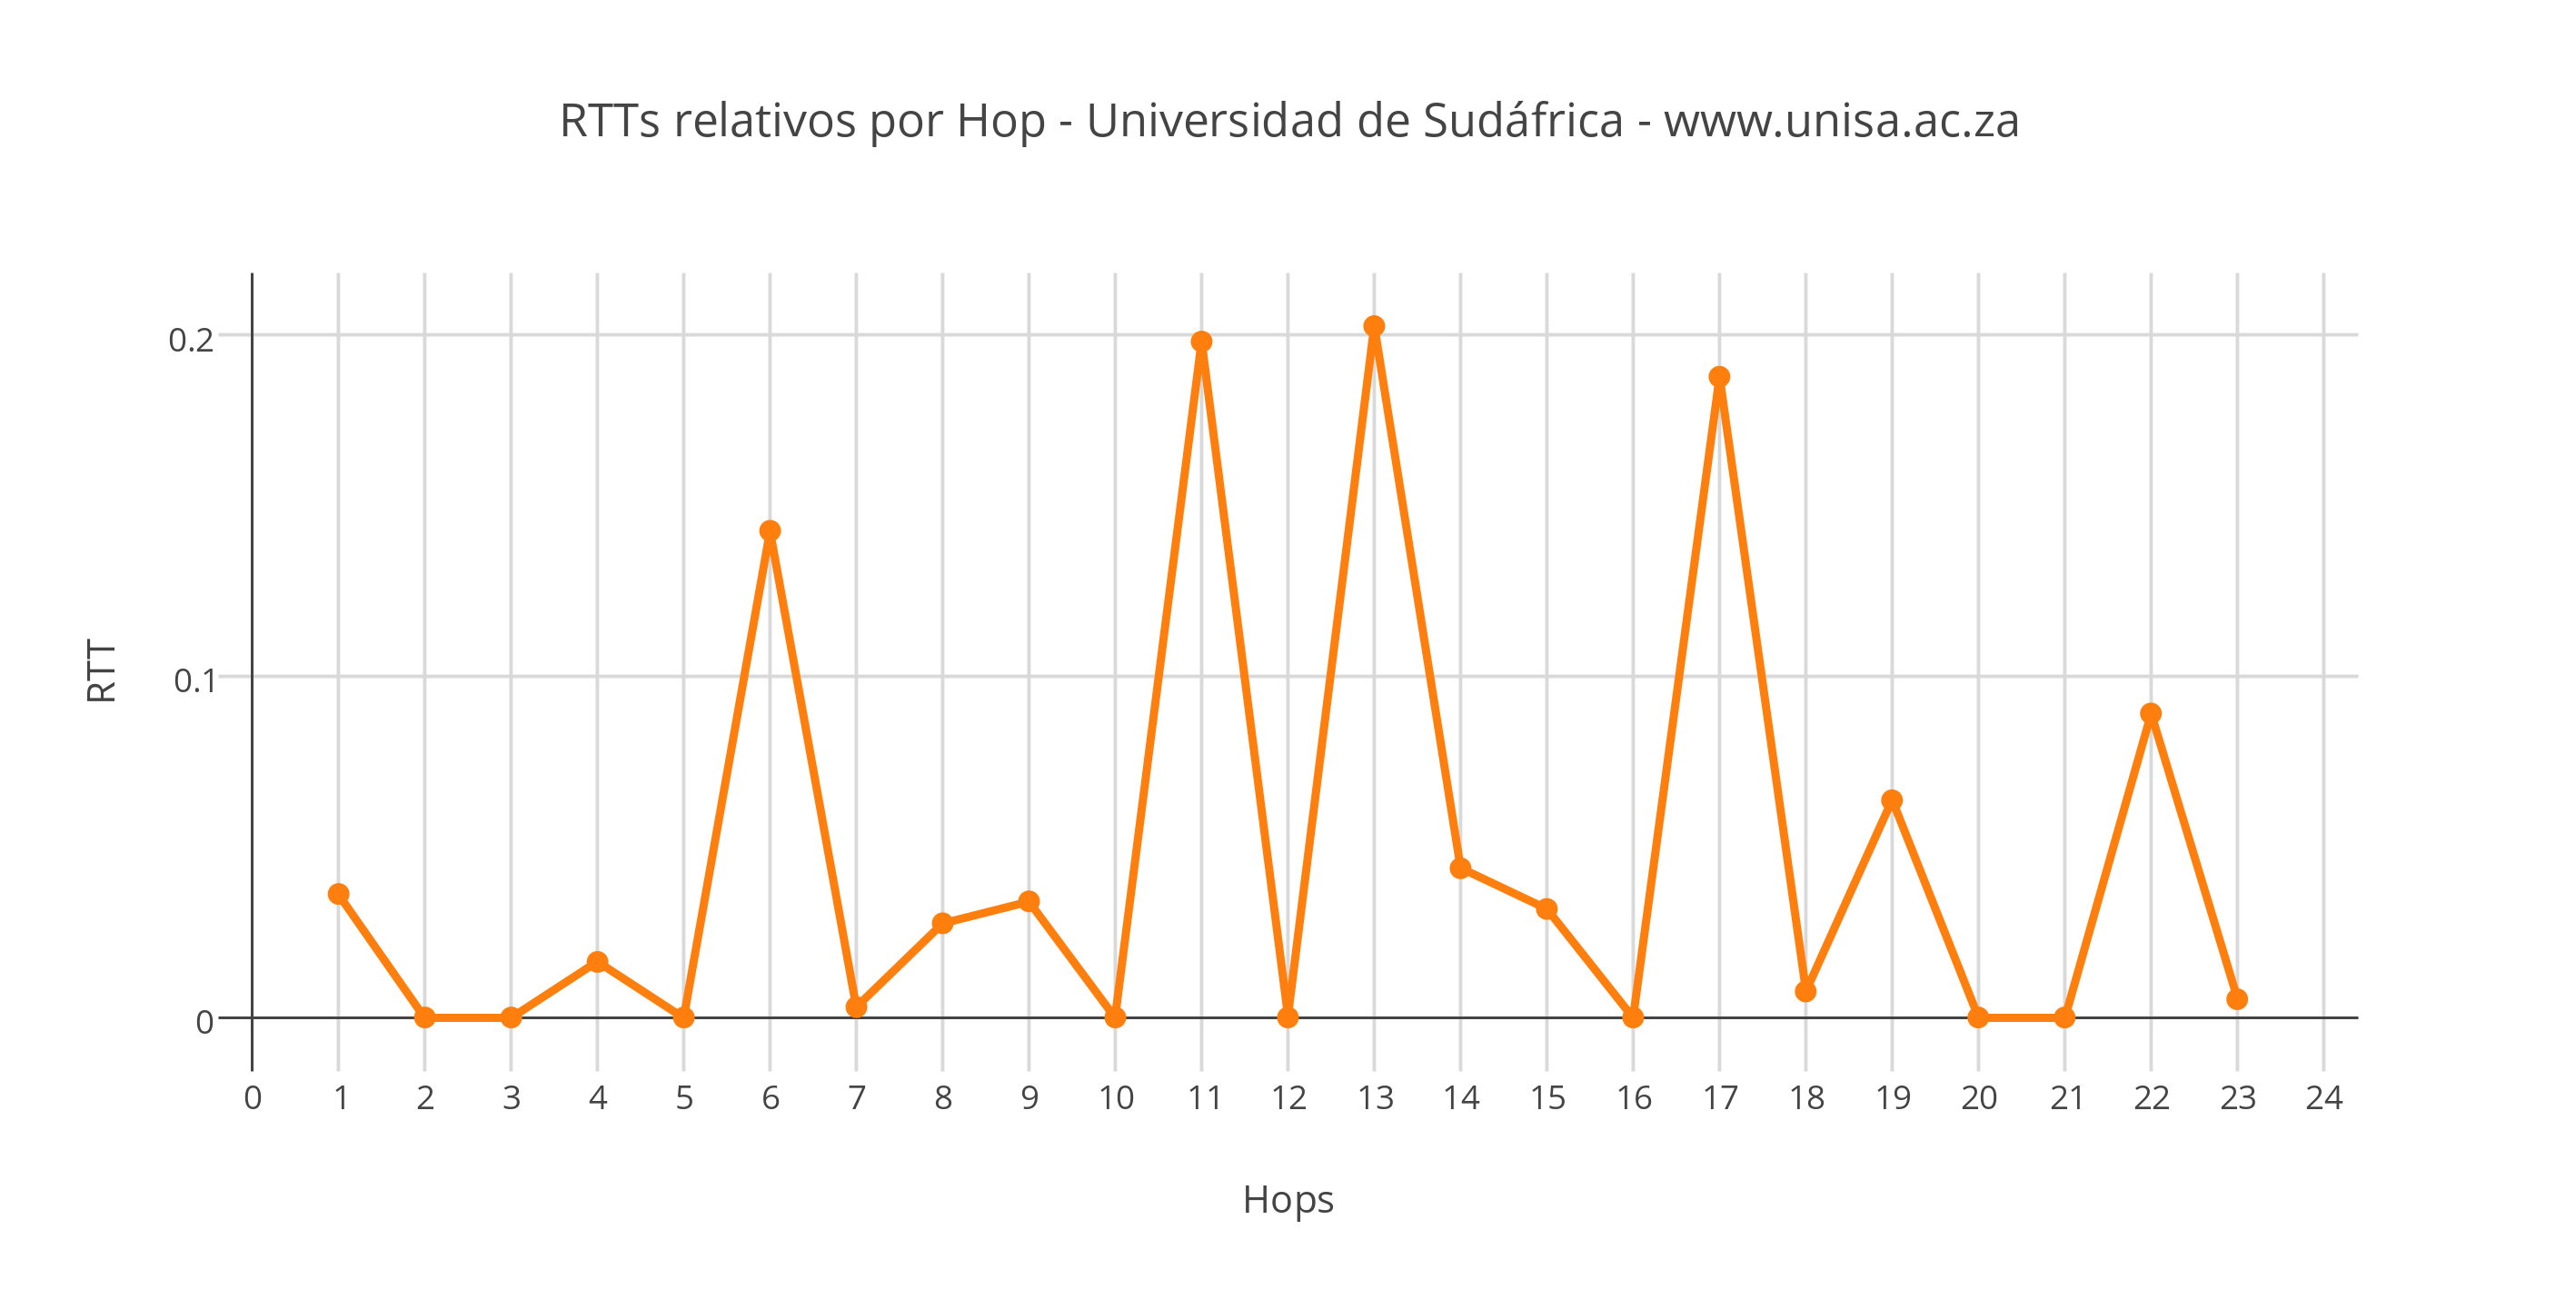
\includegraphics[scale=0.65]{imagenes/sudafrica/RTTs.png} 

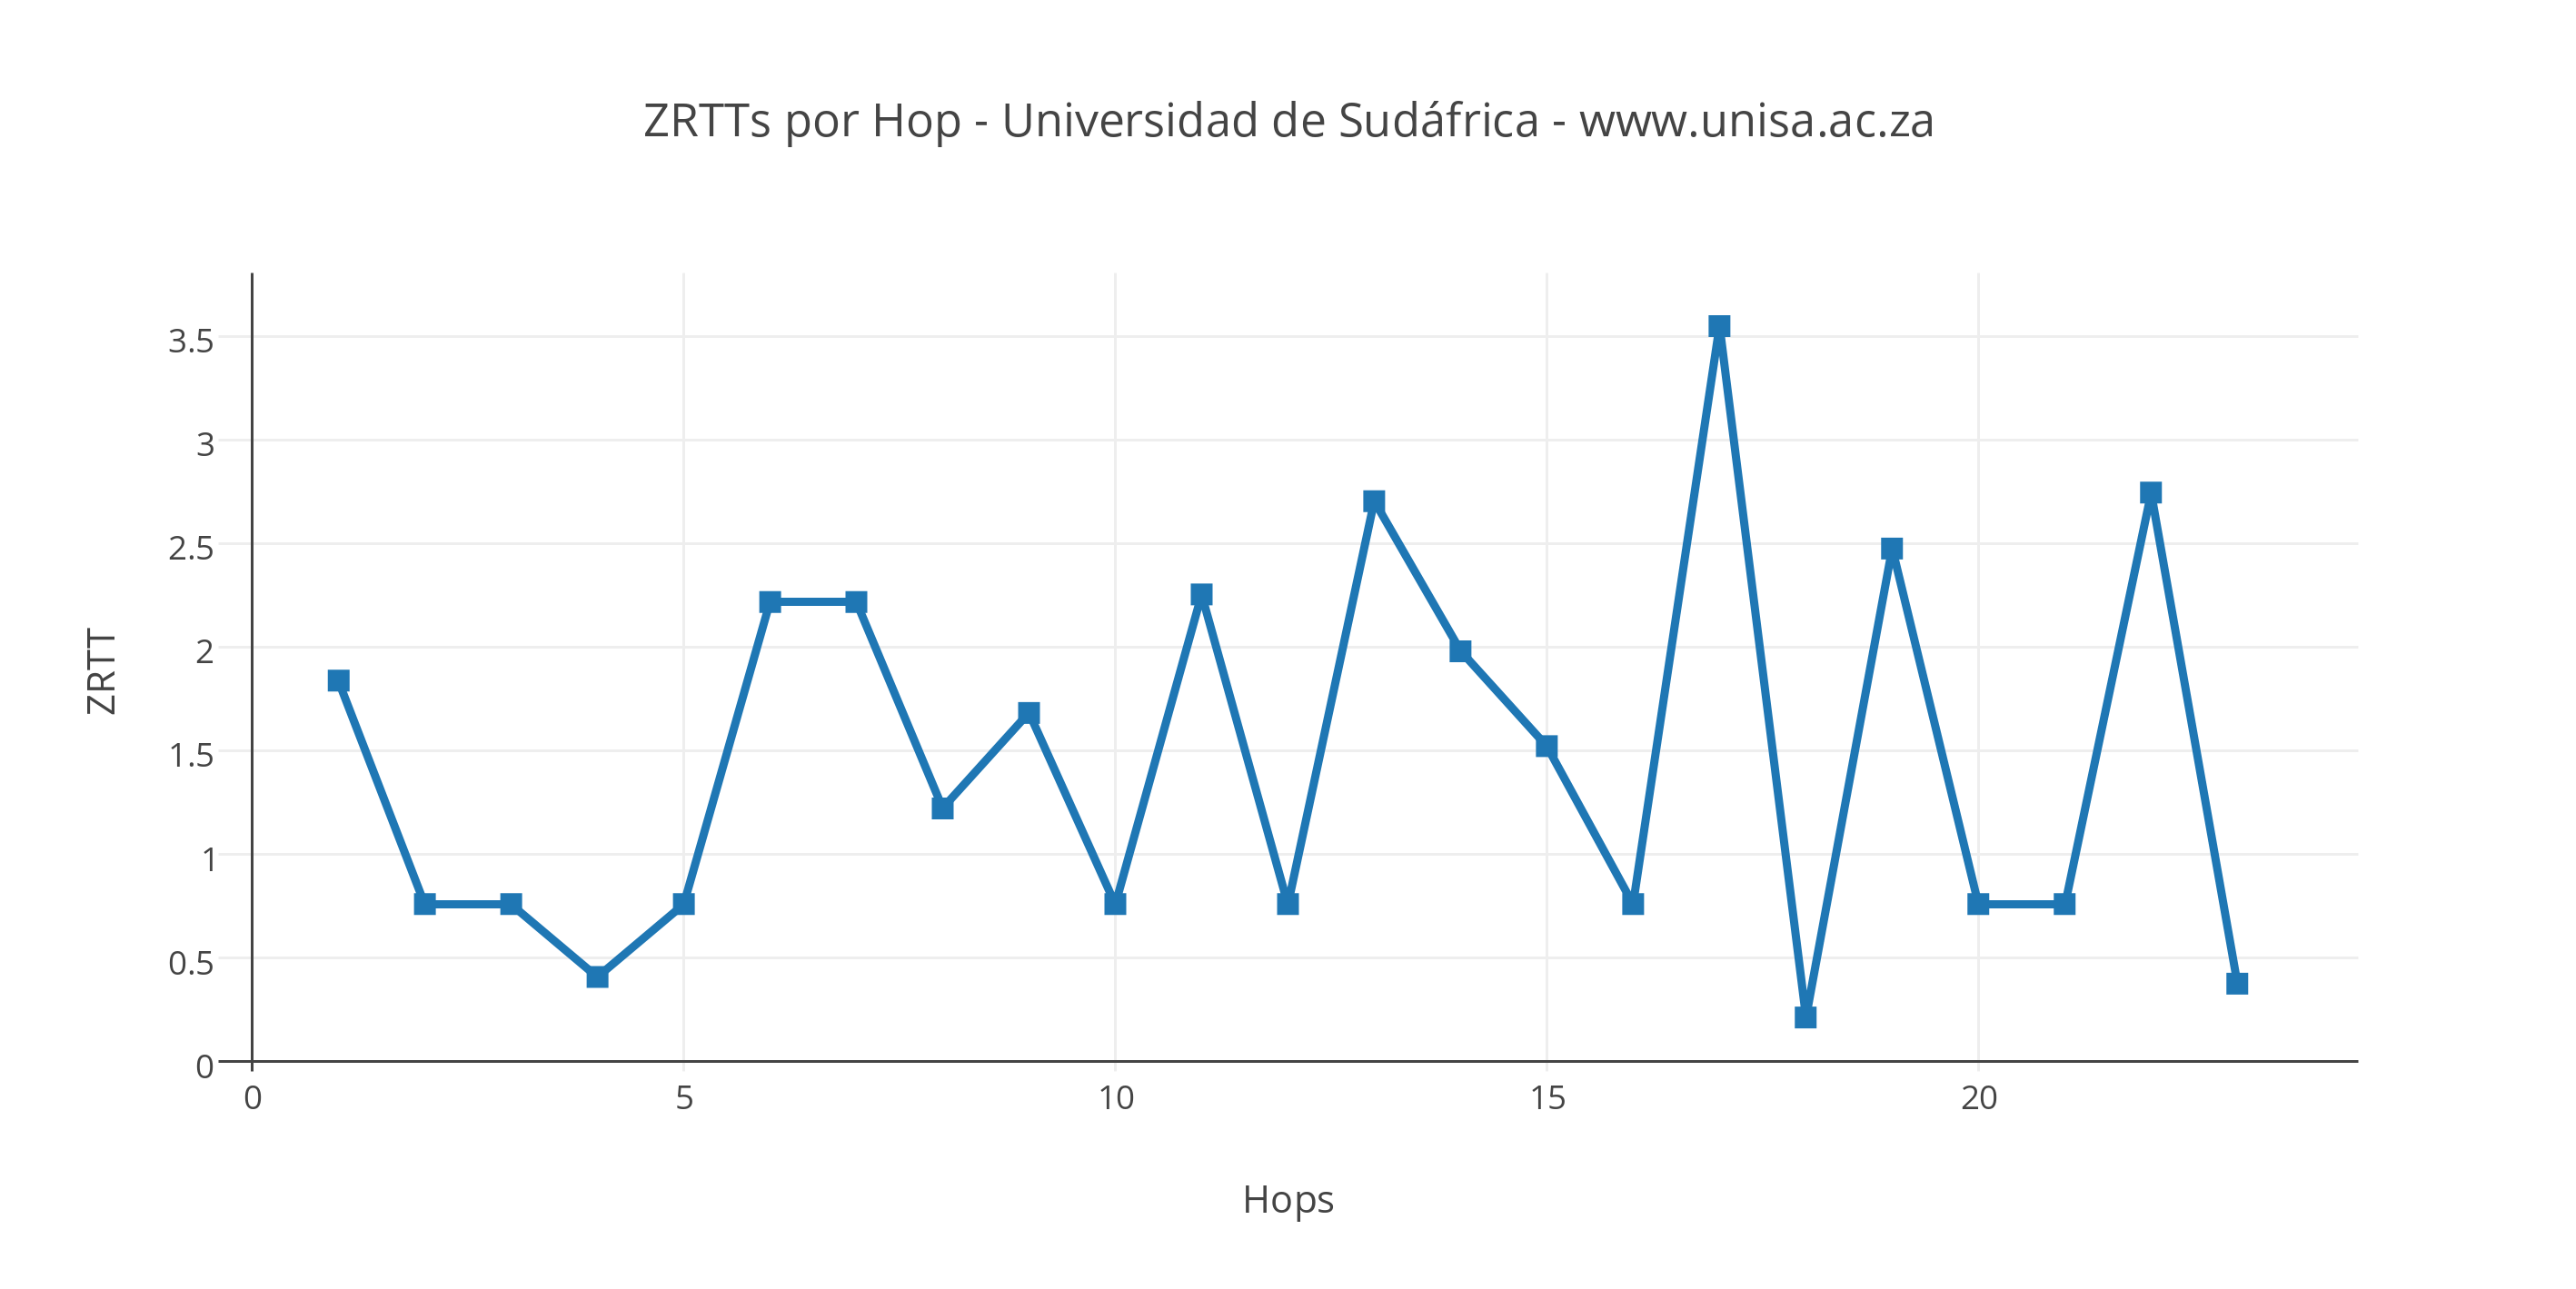
\includegraphics[scale=0.65]{imagenes/sudafrica/ZRTTs.png}

\begin{center}
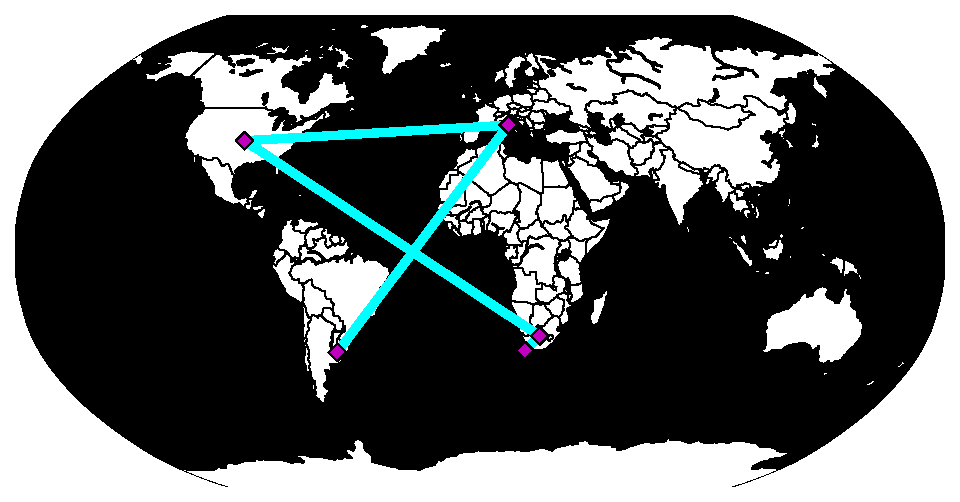
\includegraphics[scale=0.8]{imagenes/sudafrica/sudafrica.pdf} 
\end{center}
\newpage

\section{Conclusiones}

En todos los casos de monitoreo observamos la anomalía típica de los \textit{Missing Hops}. Esto probablemente se deba a que ciertas redes están protegidas por firewalls. Comparando nuestros resultados con los de la herramienta \textit{traceroute}, vimos que ésta se encontraba ante los mismos problemas. También, de manera no sorprendente, nos encontramos con la anomalía \textit{Missing Destination}, muy similar a la anterior. Para esto nos basamos en que por ejemplo, en el caso de Helsinki, los últimos hops que responden se encuentran en Finlandia, seguidos de una serie de hops que no responden. Dado que la mayoría de las Universidades cuentan con firewalls, asumimos que el paquete llegó a destino pero los firewalls no permiten que se respondan los paquetes ICMP.

También creemos habernos encontrado con anomalías del tipo \textit{False Rountrip Time}. Esta anomalía es más difícil de aseverar, pero por los picos encontrados en los gráficos de $\Delta RTT$ promedio, creemos que estamos ante un caso de esta anomalía, lo cual en algunas ocasiones pudimos verificar también con \textit{traceroute}.

Otra anomalía que encontramos fue la de \textit{Loops and Circles}, por ejemplo en el caso de la Universidad de Pekín, con los hops 6 y 7; la de San Petersburgo, en los hops 10 y 11; y en la Universidad de Sudáfrica, en los hops 6 y 7 (que parecerían estar en la misma red que los hops 6 y 7 de la Universidad de Pekín).

Creemos que no es posible mejorar demasiado la estimación de outliers del método Cimbala con un valor fijo, ya que con los valores de la tabla observamos una amplia variedad en la cantidad de outliers detectados. En algunos casos, como el de la Universidad de Helsinki, consideramos que los outliers detectados son de interés, mientras que en otros casos, como el de la Universidad de Pekín se detectan demasiados outliers, muchos de los cuáles creemos que son falsos positivos. No creemos que con un valor fijo se pueda mejorar demasiado esto; podrá disminuir la cantidad de outliers en la Universidad de Pekín, probablemente a costa de perder outliers de interés en la Universidad de Helsinki.
\newpage

\section{Referencias}

\begin{enumerate}
\item http://www.mne.psu.edu/cimbala/me345/Lectures/Outliers.pdf
\item https://www.net.in.tum.de/fileadmin/TUM/NET/NET-2012-08-1/NET-2012-08-1_02.pdf
\item http://freegeoip.net/json/
\item https://en.wikipedia.org/wiki/Outlier#Modified_Thompson_Tau_test
\end{enumerate}


\newpage

\bibliographystyle{plain}
\bibliography{tp3}

\end{document}
